\documentclass{report}

\usepackage{graphicx}
\usepackage{caption}
\usepackage{subcaption}
\usepackage{amsmath}
\usepackage{amsfonts}
\captionsetup{justification=centerlast, margin=0.5cm}
\usepackage{verbatim}
\usepackage{etoolbox}
\usepackage{mathptmx}
\patchcmd{\abstract}{\scshape\abstractname}{\textbf{\abstractname}}{}{}

\usepackage[latin1]{inputenc}
\usepackage{tikz}
\usetikzlibrary{shapes,arrows}

%\usepackage{fancyhdr}
%%\pagestyle{empty}
%
%\pagestyle{fancy}
%\fancyhf{}
%\fancyheadoffset{0cm}
%\renewcommand{\headrulewidth}{0pt} 
%\renewcommand{\footrulewidth}{0pt}
%\fancyhead[R]{\thepage}
%\fancypagestyle{plain}{%
%  \fancyhf{}%
%  \fancyhead[R]{\thepage}%
%}

\begin{document}

\title{Document Decomposition into Geometric and Logical Layout}
\date{}
\author{
  Vincent Deo\\
  Stanford University\\
  \texttt{vdeo@stanford.edu}
  \and
  Terry Kong\\
  Stanford University\\
  \texttt{tckong@stanford.edu}
  \and
  Maisy Wieman\\
  Stanford University\\
  \texttt{mwieman@stanford.edus}
}

\maketitle

\begin{abstract}
We present an Android application for scanning LaTeX documents to determine the logical layout of the document. The algorithm first prepares the image for processing, then determines where text and figures are within a document, and finally classifies these various components of a document. 
\end{abstract}

\chapter{Introduction}
One popular method of producing aesthetically pleasing PDF documents including diverse contents is LaTeX. LaTeX is a low-level markup and programming language that allows high flexibility for designing placement of text and figures, as well as overall document structure. However, this precision is hard to reproduce; once a PDF document is generated, there is no way in general to access the code used to generate the document. In particular, it is very difficult to recreate the template used to design a document. This project aims to analyze the layout of a PDF document in order to simplify the generation of LaTeX templates. 

Images are taken on an Android device and sent to a server to be processed\footnote{This is the typical pipeline for image processing tasks and is preferred in this project because of the computationally intensive tasks.}. Once sent to the server, it is processed in a combination of Matlab and Java, and the final output is saved on the server. The algorithm is comprised of 3 main steps: preprocessing, detecting maximal white rectangles, and classifying components of the document. 

\tikzstyle{block} = [rectangle, draw, fill=blue!20,text width=6em, text centered, rounded corners, minimum height=4em]
\tikzstyle{line} = [draw, -latex']


\begin{tikzpicture}[node distance = 2.8cm, auto]
% Place nodes
\node [block] (droid) {Android image capture};
\node [block, right of=droid] (binarize) {Binarization};
\node [block, right of=binarize] (skew) {Skew Correction};
\node [block, right of=skew] (margin) {Margin Removal};
\node [block,below of=margin] (mwrCC) {Preprocess Connected Components};
\node [block, left of=mwrCC] (mwrTree) {Maximal White Rectangles};
\node [block, left of=mwrTree] (mwrPost) {Postprocess White Rectangles};
\node [block, left of=mwrPost] (proj) {Analyze Horizontal Projections};
\node [block, below of=proj] (feat) {Global and Local Feature Comparison};
% Draw edges
\draw[->] (droid) -- (binarize);
\draw[->] (binarize) -- (skew);
\draw[->] (skew) -- (margin) ;
\draw[->] (margin) -- (mwrCC);
\draw[->] (mwrCC) -- (mwrTree);
\draw[->] (mwrTree) -- (mwrPost);
\draw[->] (mwrPost) -- (proj);
\draw[->] (proj) -- (feat);

\end{tikzpicture}

\chapter{Preprocessing}
Before analyzing the image, a reliable binarized representation of the image must be found to allow for proper interpretation of various components of a document. To optimally apply further document analysis, the image must be vertically aligned without a background. The image is captured with a mobile phone, and the document in the picture may be rotated or have low contrast. This section discusses our method of addressing these concerns in order to prepare the image for layout analysis.

\section{Binarization}
Lighting conditions may be uneven, so adaptive Otsu thresholding is used to binarize segments of the image. Overlapping windows of a fixed size are applied to the image, and for each window, the variance is compared to some threshold to determine whether to apply the Otsu threshold. This threshold is partially determined by the mean and variance of the entire image, since images that are taken with low lighting levels will have lower means and variances. After computing for each window, any pixels that have been evaluated as black more than twenty percent of the time are determined to be black.

\section{Skew Detection}
Images taken at an angle must be rotated so that text lines are parallel to the image edges. The Hough transform is used to determine the angle to which the image is rotated. Rather than applying the Hough transform to the whole image (which will detect lines that stretch diagonally across text, as well as dominant lines in the background), we apply the Hough transform to smaller portions of the image. We determine which regions are most likely to be text by evaluating the variance, and we take the Hough transform of regions where the variance is high.  


For each window, we find the histogram of angles, and sum the contributions. We assume that the image will be rotated by an angle less than forty-five degrees. Because of this, we can combine the contributions of perpendicular lines; a page with text going in one direction will often have lines perpendicular to the text, whether those lines represent the edges of the paper or the edges of figures. When the input angle is constrained, we can interpret perpendicular lines as representing the same input angle. We rotate the image by the angle that occurs most often in this new histogram of combined perpendicular lines.

\begin{figure}%
\setcounter{subfigure}{0}
\centering
\begin{subfigure}{.45\columnwidth}
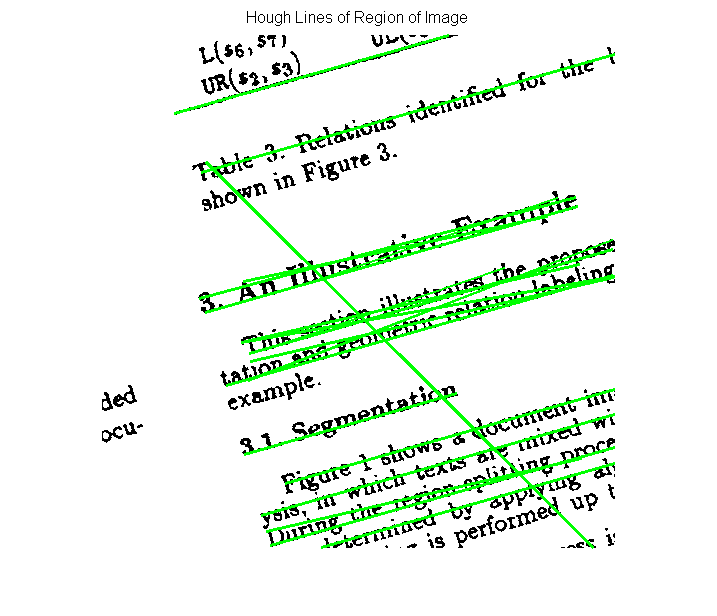
\includegraphics [width=\columnwidth]{HoughLinesEx.png}
\subcaption{Detecting Hough Transform lines of small portions of an image.}
\end{subfigure}
\hfill%
\begin{subfigure}{.5\columnwidth}
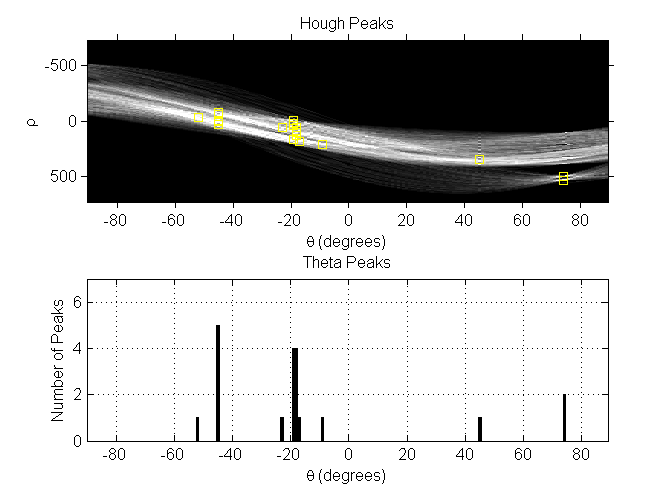
\includegraphics [width=\columnwidth]{HoughPeaksEx.png}
\subcaption{Theta Values of Hough Peaks}
\end{subfigure}
\end{figure}

\section{Background and Margin Removal}
To remove the background, we find the edges of the document. If the background is in contrast with the paper, binarization will detect high variance at the edges of the document, and create dark edges around the document. We find these dark edges by creating a histogram detailing the longest consecutive line of dark pixels for each row and column, and find where the number consecutive dark pixels is greater than average, which occurs at the longer stripes across the edges. Once we have determined the boundaries of the paper, we must then remove the margin. We then apply a median filter to denoise the image, and find the first and last rows and columns with black pixels to remove the margin.



\chapter{Layout extraction by Maximal White Rectangle analysis.}

\section{Approach and Purpose}
% Where it comes from
The Maximal White Rectangles (MWR) approach for document layout analysis was developed by Henri S. Baird in the 90s. With recent dramatic
improvements in computing power, this technique formerly either very constrained or very slow is now achievable for full scale 150 to
300 dpi binarized documents.\\

The idea of MWR analysis comes from a global-to-local, non-backtracking document analysis approach matching the implicit approach of a human
reader. Indeed, the eye is first attracted to important white spacing from which we deduce the reading order. e.g first the margins, then isolate
the title, separate the columns of text, then the paragraph boundaries, etc. Similarly, the MWR algorithm enumerates all the maximum (by inclusion
order) empty rectangles, in a document image, and outputs them sorted by an area-based metric.\\

From that point, we are to select a given percentile of the highest-scoring MWRs, which reunion creates a template of empty zones in the original
images (see figure \ref{MWRoverlayEx}). The remaining area uncovered by selected MWRs is separated in connected components which are likely
to correspond to logical blocks in the document, given that they are surrounded by large empty areas but do not contains such large white areas.\\

The purpose of the MWR in this context is to use this overlay, to further on use the relative positions of the blocks to determine their reading
order and logical functions.

\begin{figure}
\centering
\begin{subfigure}{0.47\textwidth}
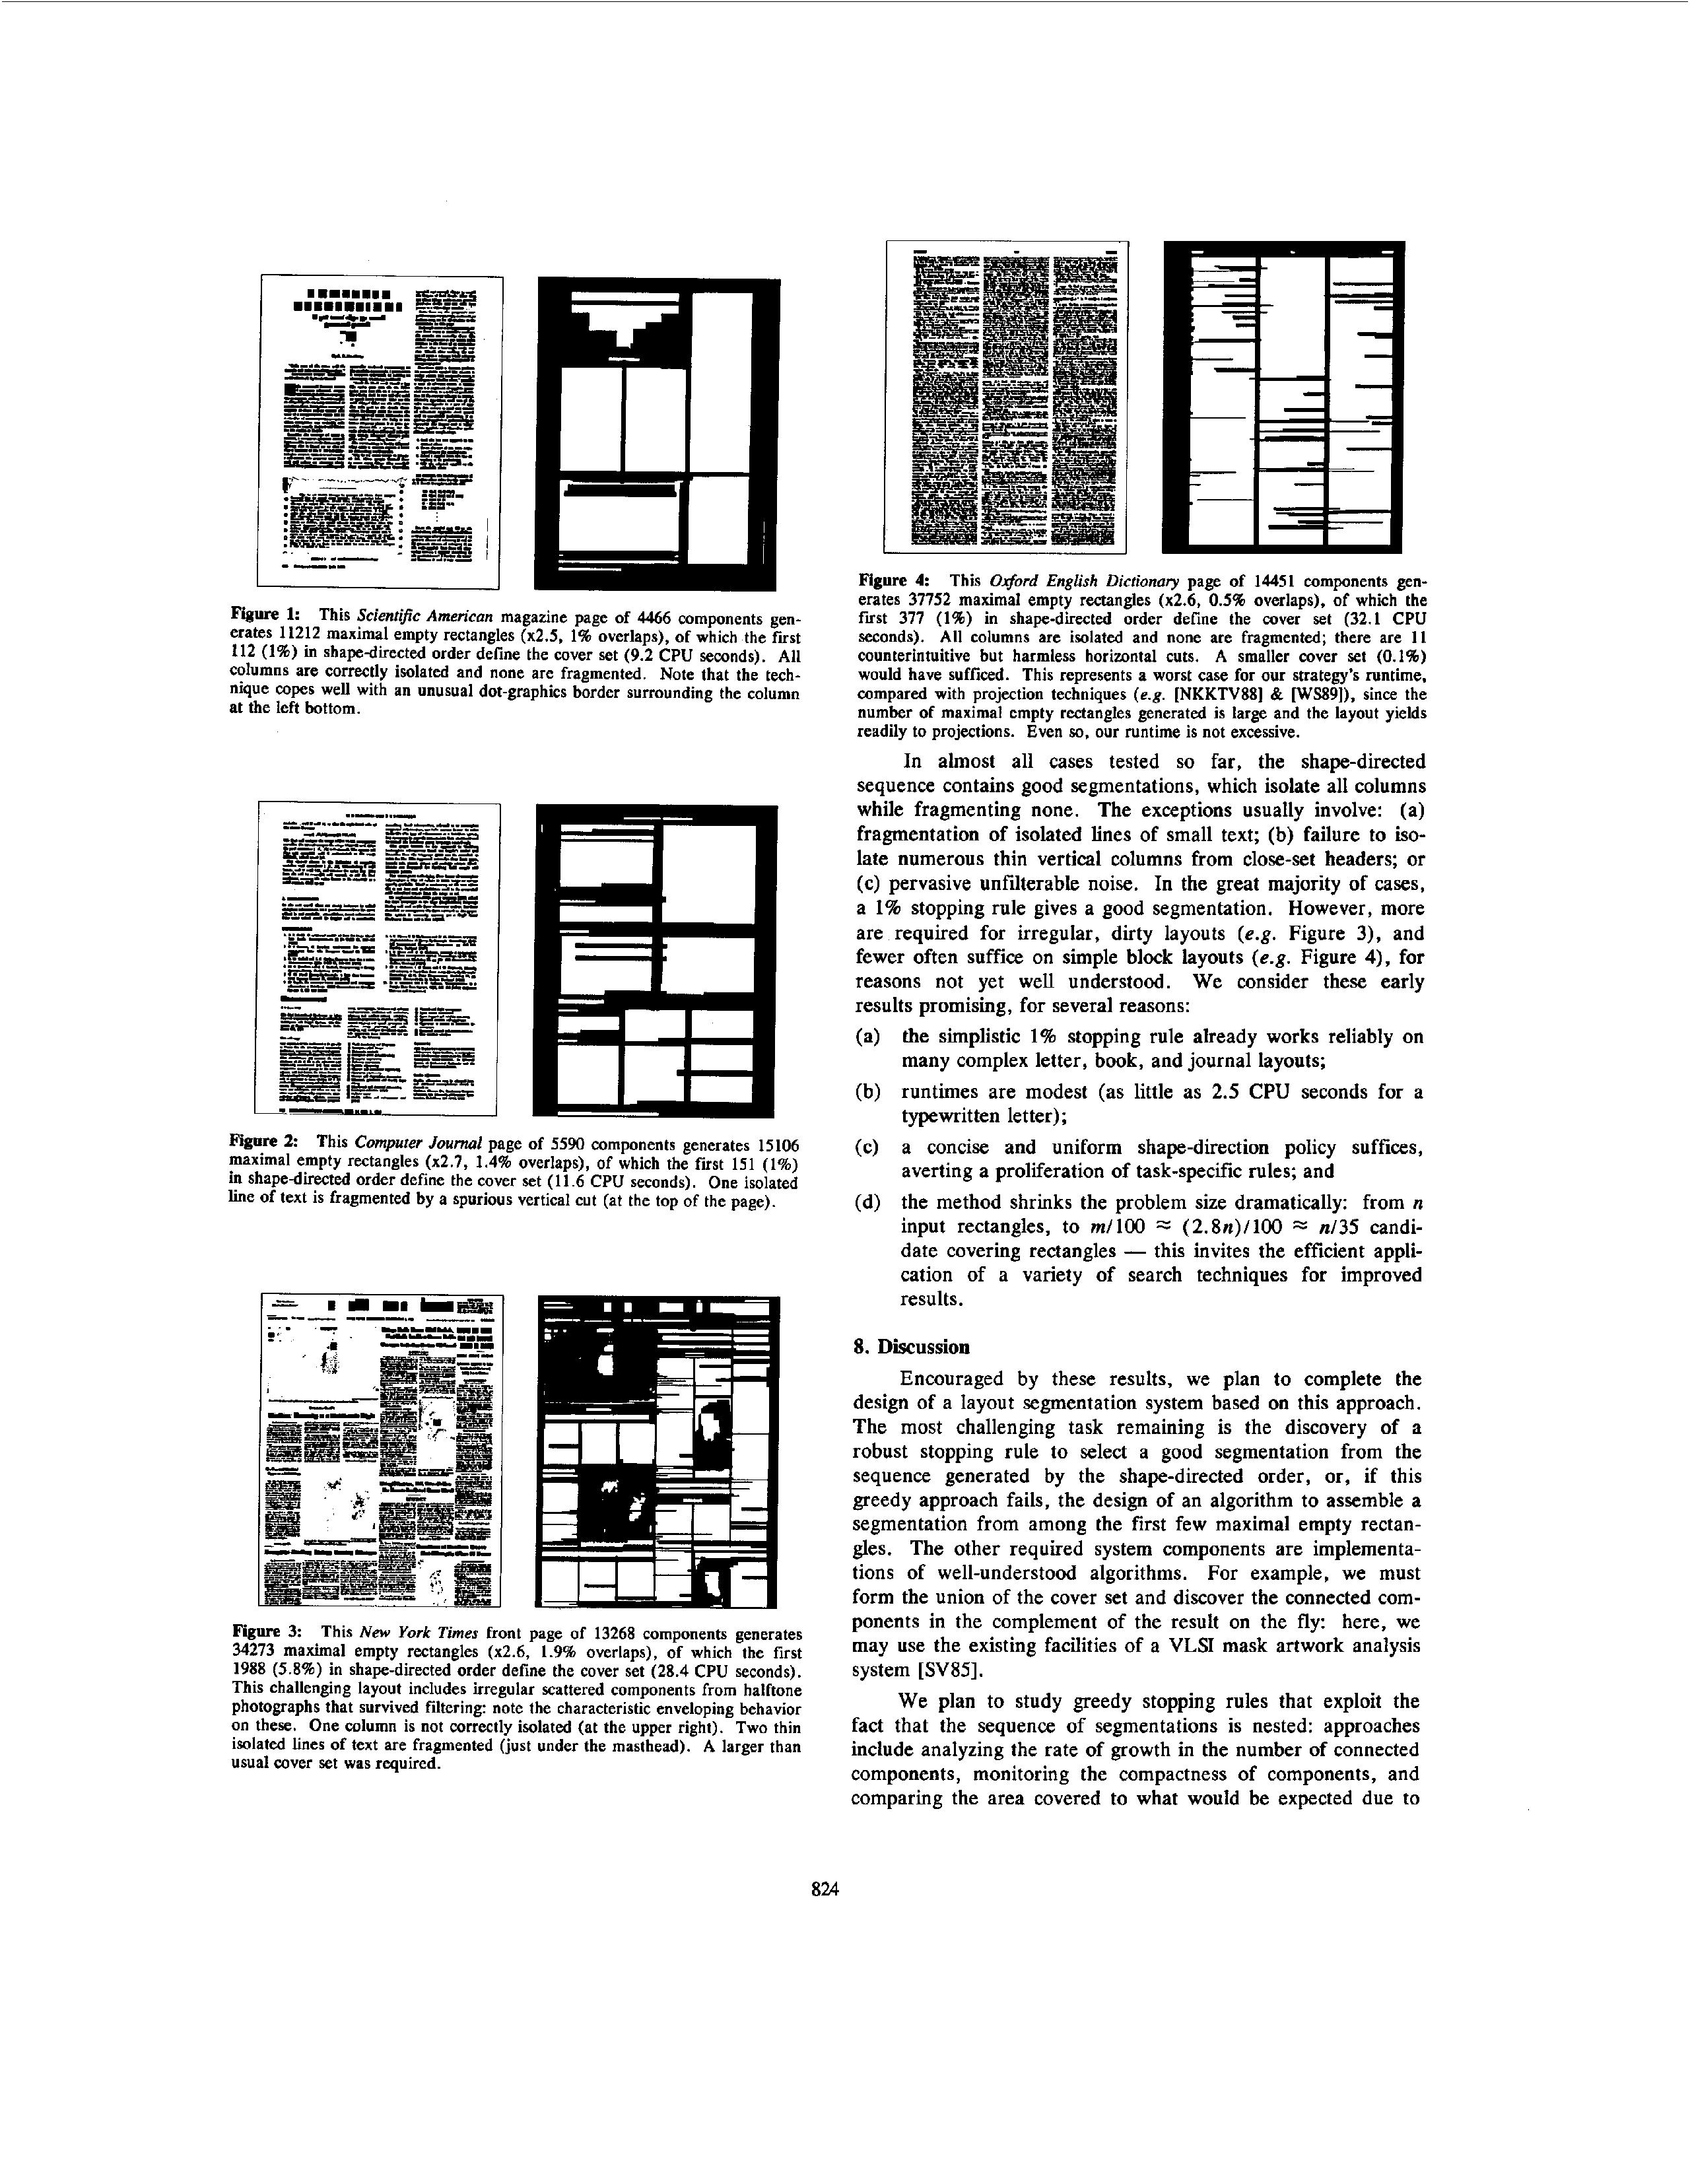
\includegraphics[width = \textwidth]{document1.png}
\end{subfigure}
\hspace*{0.03\textwidth}
\begin{subfigure}{0.47\textwidth}
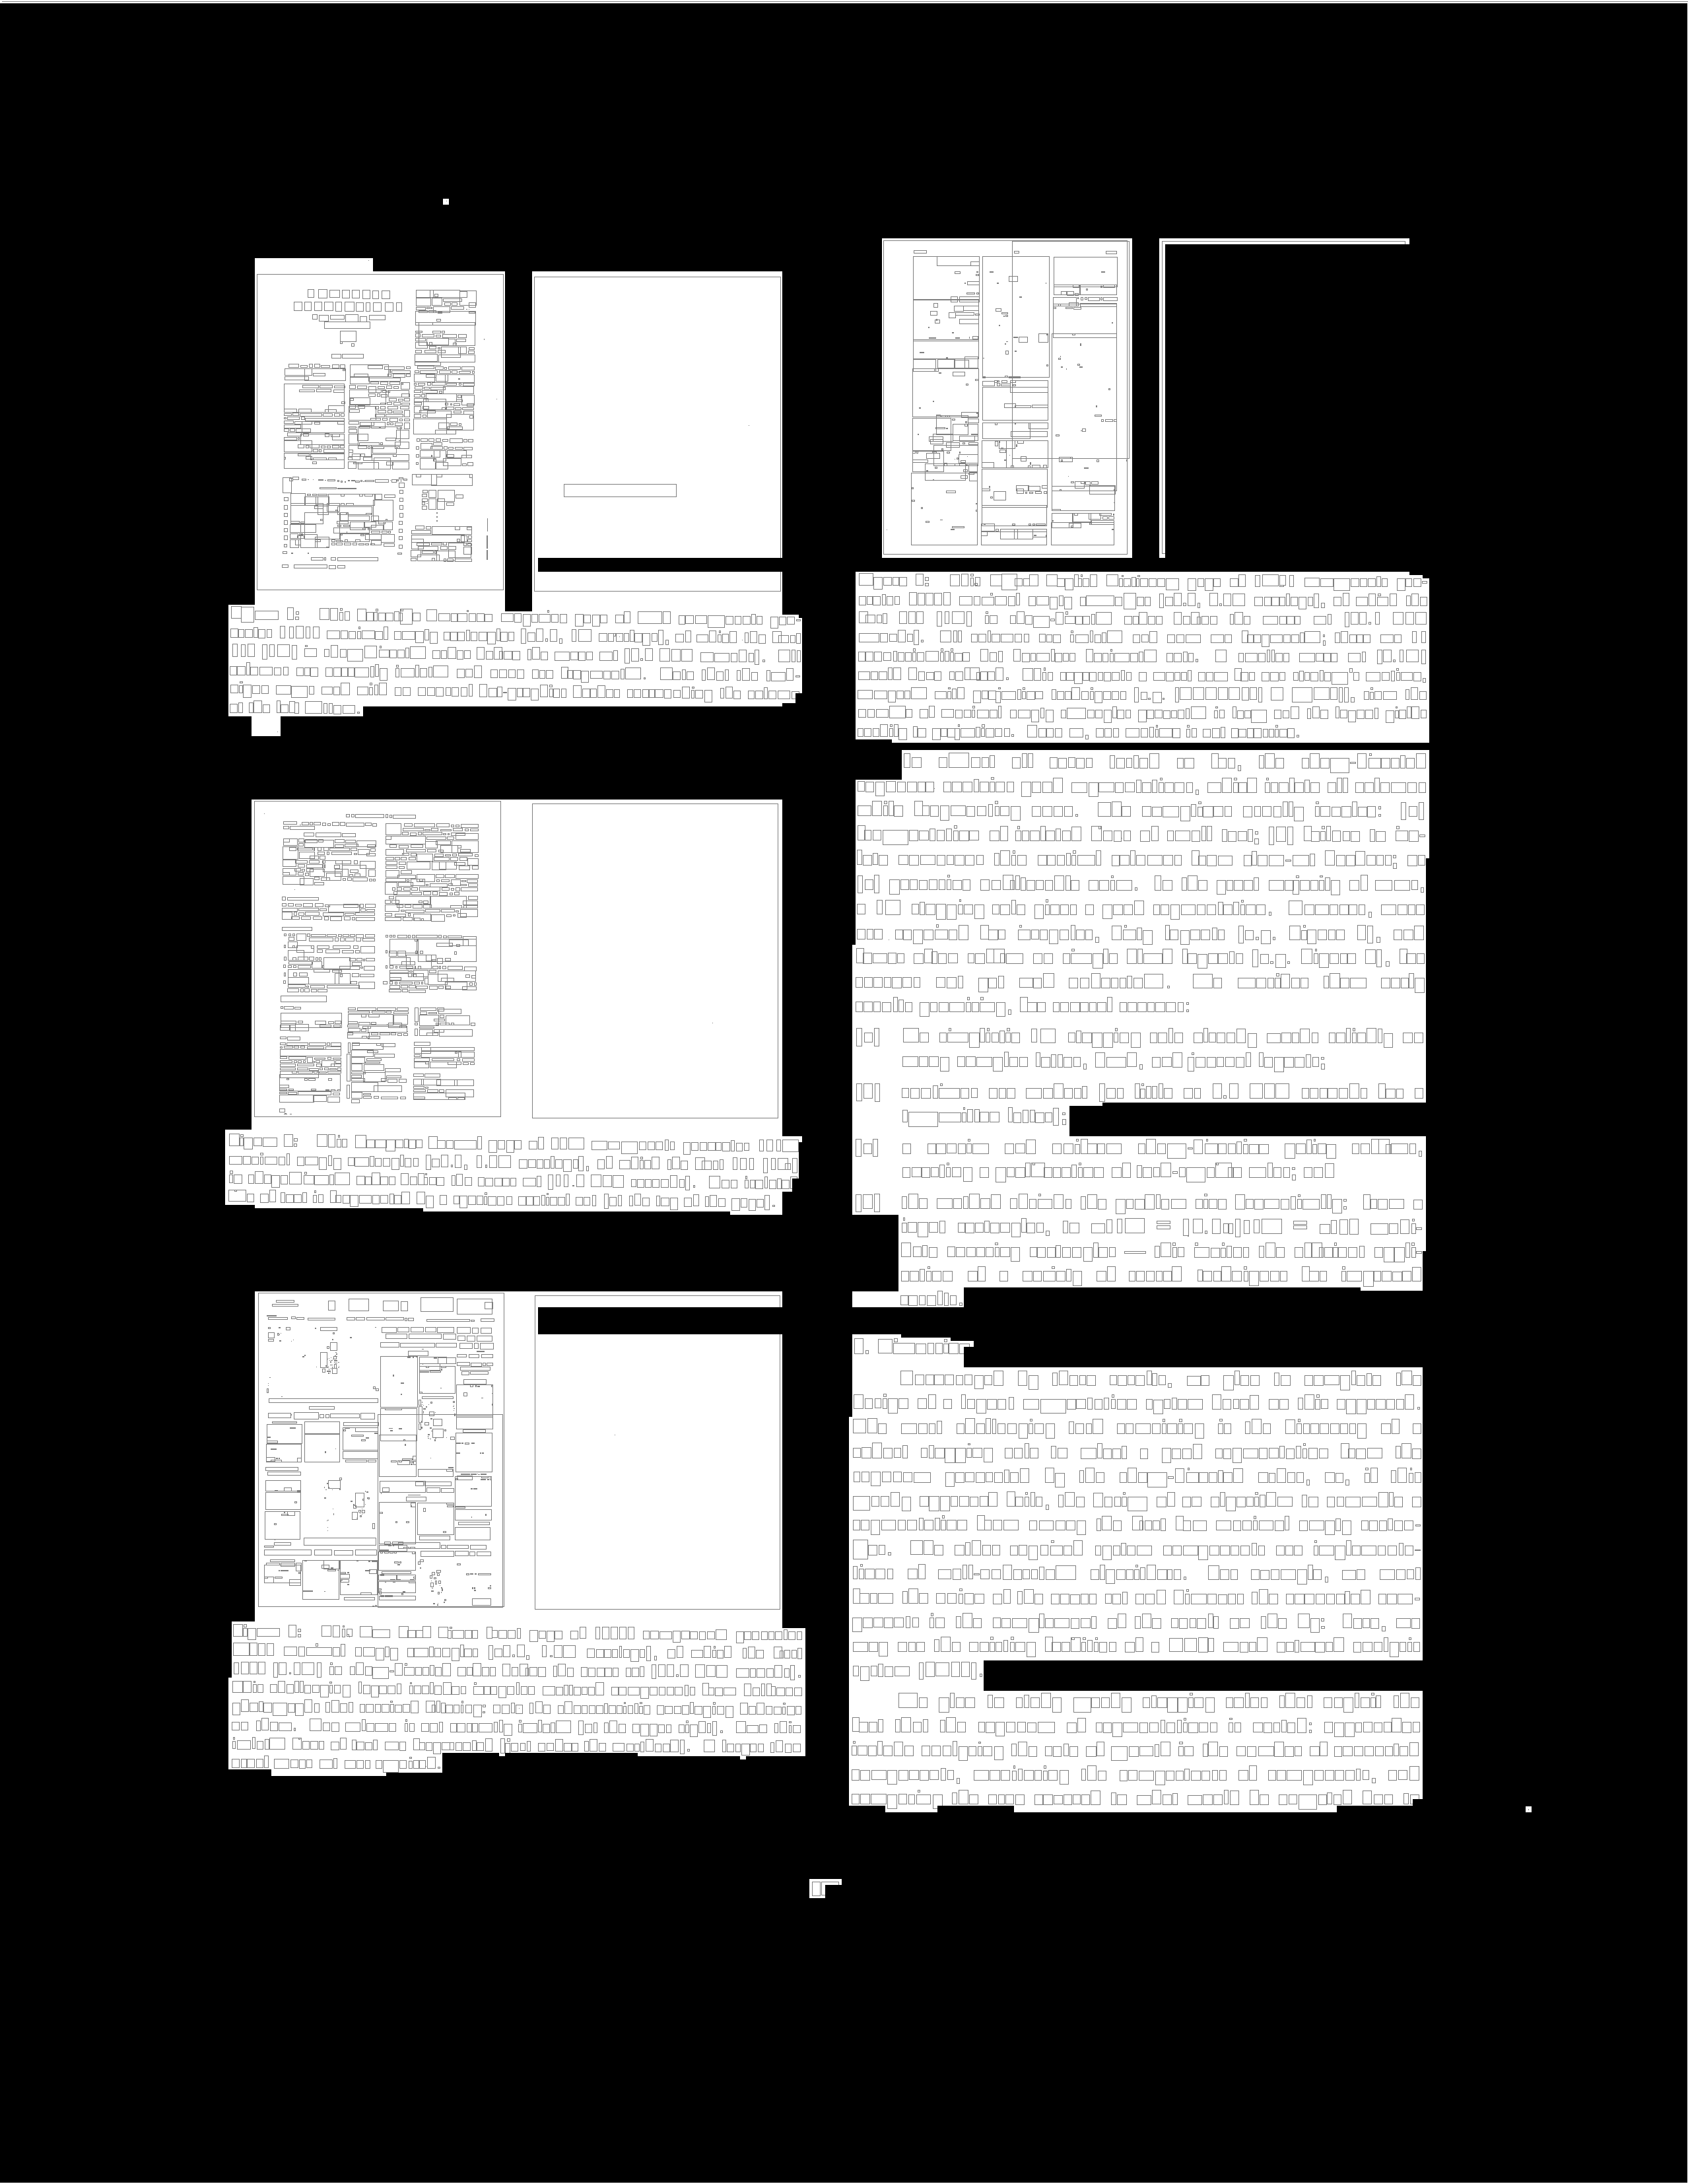
\includegraphics[width = \textwidth]{overlay1.png}
\end{subfigure}
\caption{Left: a typical document. Right: Its generated overlay with MWR enumeration. Rectangles going through figures are a preprocessing
artifact which is corrected further in the processing.}
\label{MWRoverlayEx}
\end{figure}

\section{Algorithm}
The algorithm used to enumerate all the maximum white rectangles in a binary image is described in this section. It is a balanced-tree-based
algorithm, which overall complexity is $\mathcal{O}(n\log(n))$ where $n$ is the number of maximum white rectangles, which itself
amounts to $\mathcal{O}(m^2)$ in the worst case with $m$ the number of black pixels.\\

\subsection{Preprocessing}
For runtime reduction, we use a connected-component reduction pre-processing. Each black connected component is extracted from the original
image, from which we extract a pixel-aligned rectangular frame surrounding it. Only two sides of this frame are kept, the left and top ones.\\

This step reduces every connected component to a 1-pixel thin `$\Gamma$'-like shape, which then can be downsampled with very little loss of
information.
The templates of the connected components are stored for further overlaying after MWR enumeration. With that preprocessing, we achieve a
reduction of the number of black pixels to process by typically 70-80\% before downsampling, that amounts to a total reduction of 85-95\% after
downsampling.\\

A typical 300 dpi letter format document (8.5 Mpx) contains about 1,000,000 black pixels in 10,000 connected components, which is
reduced to a preprocessed image of 1 Mpx with 50,000 - 150,000 black pixels.

\subsection{MWR Enumeration Core Algorithm}

The algorithm sweeps across the document from left to right, processing all black pixels. The pending maximal white rectangles are kept in a
balanced tree structure in which every node represents a rectangle. Such a rectangle is represented by its upper, lower and leftmost bound, until
a black pixel interrupts the rectangle by imposing a right bound.\\

The tree structure is naturally derived from a natural point of view of creating maximal white rectangles sweeping from left to right.
`Thin' white rectangles go from the left margin to the current column in between the already found black pixels. Taller rectangles start at the
right of already processed black pixels. See figure \ref{rectangles}.

\begin{figure}
\centering
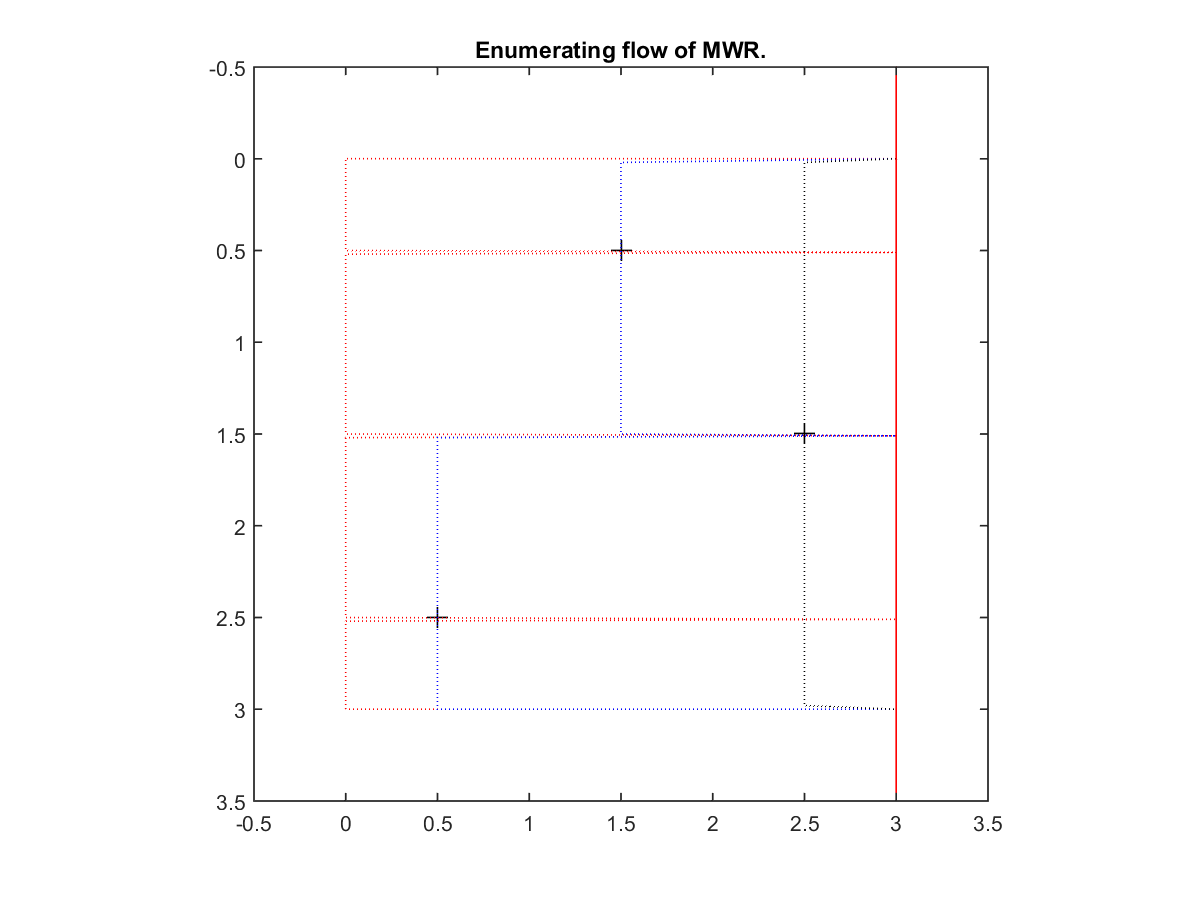
\includegraphics[width = 0.9\textwidth]{rectflow.png}
\caption{State of running MWR enumeration. Solid red: column being processed, Black crosses: black points/pixels. Black dotted: rectangle root of
the tree. Blue dotted: rectangles of depth 1 in the tree. Red dotted: leaves of the tree, corresponding to rectangles going all the way to the
left.}
\label{rectangles}
\end{figure}

The tree is kept balanced with the following invariants:
\begin{itemize}
  \item The leaves of the tree from (left to right) form an uninterrupted partition of the height of the image, all being rectangles starting at
  the left edge.
  \item the root is a rectangle covering the whole height of the paper, with its left edge starting at the last (hence rightmost so far)
  processed black pixel
  \item For any node, the leaves of the subtree below span an exact partition of the height span of the rectangle represented by this node.
  \item For any node, the left bound is larger than the left bound of all rectangles in the subtree below.
\end{itemize}
For the processing step displayed on figure \ref{rectangles}, the rectangle tree would be the following, with the syntax
\verb+([top,bottom],left)+ for a running rectangle.\\

\begin{verbatim}
                            ([0,3], 2.5)
                           /            \
             ([0,1.5], 1.5)             ([1.5,3], 0.5)
           /              \            /             \
     ([0,0.5], 0)  ([0.5,1.5],0) ([1.5,2.5],0)    ([2.5,3],0)
\end{verbatim}

The invariants described above are preserved by the following process for integrating a new black pixel:
\begin{itemize}
  \item Find the lowest node being split if the vertical direction by this black point. Discard all the nodes that are split as finished MWRs.
  \item split the tree along the split node and its fathers (that are all split as well). A rebalancing operation not described here ensures that
  the depth does not increase dramatically during these operation.
  \item Merge the two trees generated by the previous step under a new root, a rectangle starting a the current black pixel and spanning the
  whole height.
\end{itemize}

\subsection{Implementation}
It is to be noted that the algorithm described above processes ponctual black dots in a continuous 2D space. Optimizations can be done when we
know black dots are actually 1-px wide and necessarily lie on a grid. Otherwise, we just need to discard 1-unit wide rectangles as being
nonexistent (in between contiguous black pixels).\\

For performance, the algorithm was implemented in the Java language, achieving a runtime of about 8 seconds for a typical document.

\section{Post-processing}
The process allows to successively discard maximal white rectangles in a binary layout. This rectangles are immediately pushed in a priority
queue which keeps them sorted by a user-defined metric.\\
Empirically, the rectangles that best separate the logical block without going through them are the large rectangles with a large aspect ratio,
such as ones running between columns or cutting in between two paragraphs, or between a figure and its caption. For that purpose, the following
classifying metric was empirically developed by Henri S. Baird, and is the one we used in this project with encouraging results. The ceiling of
aspect ratio to 16 is somehow arbitrary but allows to avoid growing the score of -for instance- very thin rectangles that run in between
characters.
\[
\mathrm{score} = \mathrm{area} \times \log(\min(\mathrm{aspect ratio}, 16))
\]
Finally, a certain percentage has to be chosen to construct the image layout. In this project, we have used between 1-5\%, providing typical
results as shown in figure \ref{MWRoverlayEx} \footnote{This was produced with 1\% of all MWR.}. Typically our preprocessed images contain about 15,000 MWR, and between 100-200 MWR is a good
quantity to determine the block-by-block layout without separating lines with smaller rectangles.\\

After this MWR layout processing, logical components are isolated and can be analyzed either independently or together to determine their nature
and logical connections, which is done in the following steps of the project.

\chapter{Classification}
Once the maximal white rectangles have been calculated, a subset of the largest rectangles can be used as partial covers to segment content in the document. The union of these partial covers creates a mask for the document where connected components in the mask are blocks of content. It is crucial that the chosen subset of partial covers correctly separates different types of content; otherwise the classification will be meaningless.

\subsection{Assumptions} 
There are many types of document layouts that each have different conventions for properties such as caption position or footer extent. This required us to limit the scope of document layouts the algorithm may accept in order to guarantee reliable classification. Academic papers and textbook pages tend to follow the conventions that we aim to cover, but more generally, any document that follows these set of rules should be correctly decomposed and classified:

\begin{itemize}
\item The document should be in Manhattan Layout, but in general, any one type of content in the document must have a rectangle that circumscribes only that content and no other type of content.
\item Text is horizontal.\footnote{Vertical Text would be recognized as a figure.}
\item Figures must have captions, and the captions must be proximal and appear below the figure.
\item Page Numbers must be centered at the bottom of the page.
\end{itemize}


The types of content that we aim to classify with this set of rules are \textit{text, figures, captions, page numbers and miscellany objects, e.g., horizontal and vertical dividing bars.} First, a global-to-local classification is done to classify a block of content as text, figure, or neither, and then local classification is done to classify types of text.

\subsection{Global-to-Local Text Classification}
Within global-to-local classification, there are two main types of content: "large" content and "small" content. The terms "large" and "small" are loosely used here because they are qualifiers of both area and aspect ratio. More on this is discussed in subsequent sections.

\subsubsection{"Large" Content}
Given that a block of content is "large," it is almost certain that this block is either text or a figure. The approach of classifying this large block involves taking the horizontal projection and analyzing it's autocorrelation which is based off of \cite{BairdOrig}. The fundamental idea is that \emph{large blocks of text have multiple parallel lines of text which are separated by line breaks}. Once a horizontal projection is taken, it can be considered as a quasiperiodic signal. If there is a strong fundamental frequency component in this signal, which corresponds to the line break spacing, the block is considered text. The blue line in the plot Figure \ref{texthist} is an example of a horizontal projection of a block of text.

\begin{figure}%
\setcounter{subfigure}{0}
\centering
\begin{subfigure}{.33\columnwidth}
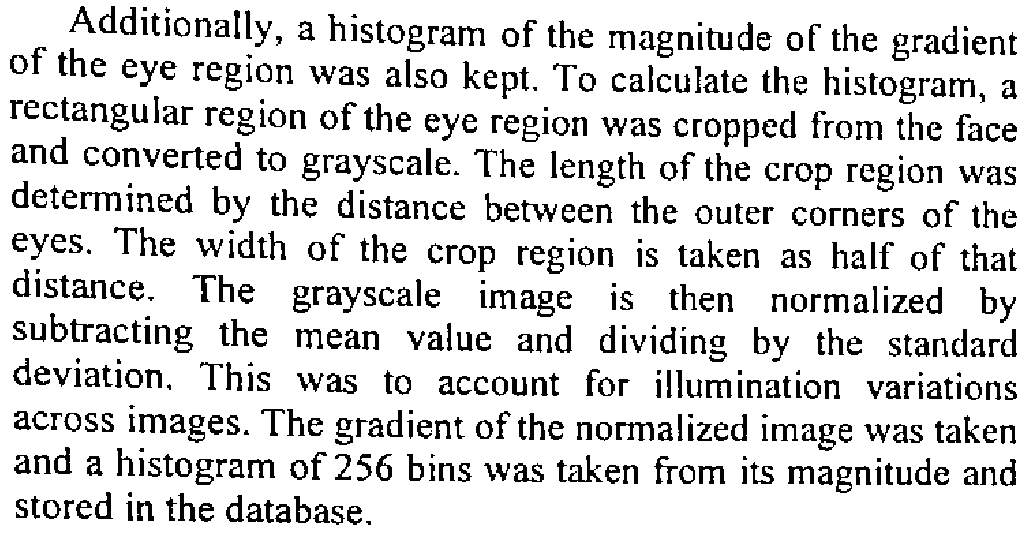
\includegraphics[width=\columnwidth]{textblock.png}%
\subcaption{Text Block}
\label{textblock}
\end{subfigure}\hfill%
\begin{subfigure}{.33\columnwidth}
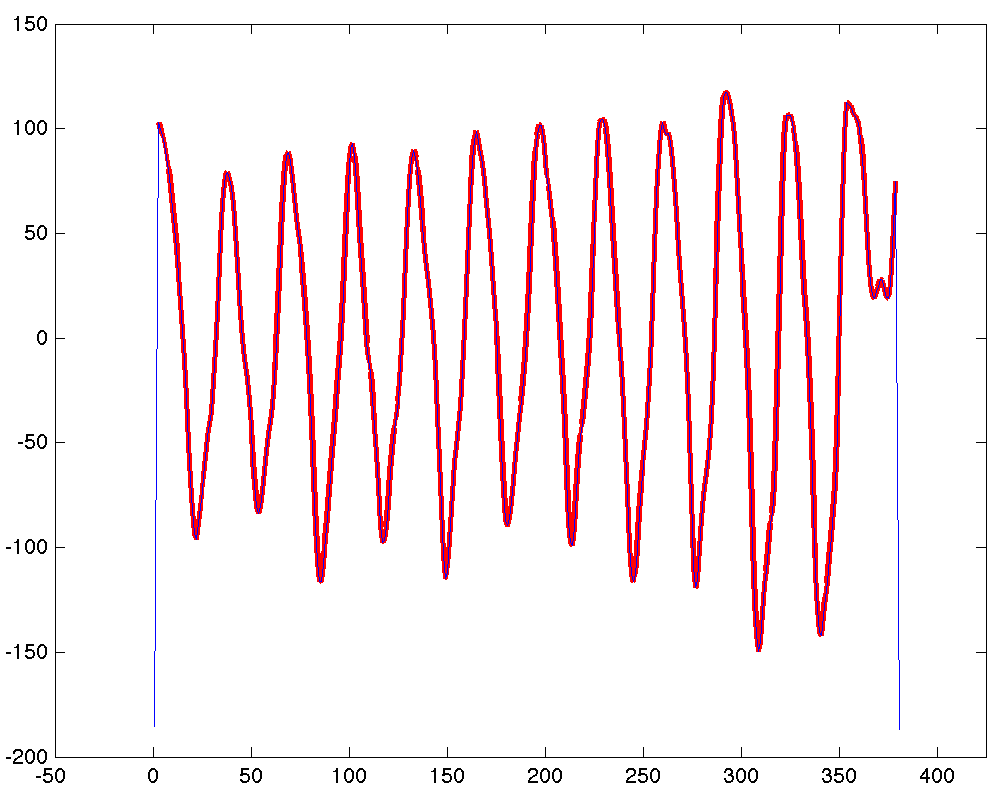
\includegraphics[width=\columnwidth]{texthist.png}%
\subcaption{Text Block: Horizontal Projection}
\label{texthist}
\end{subfigure}
\begin{subfigure}{.33\columnwidth}
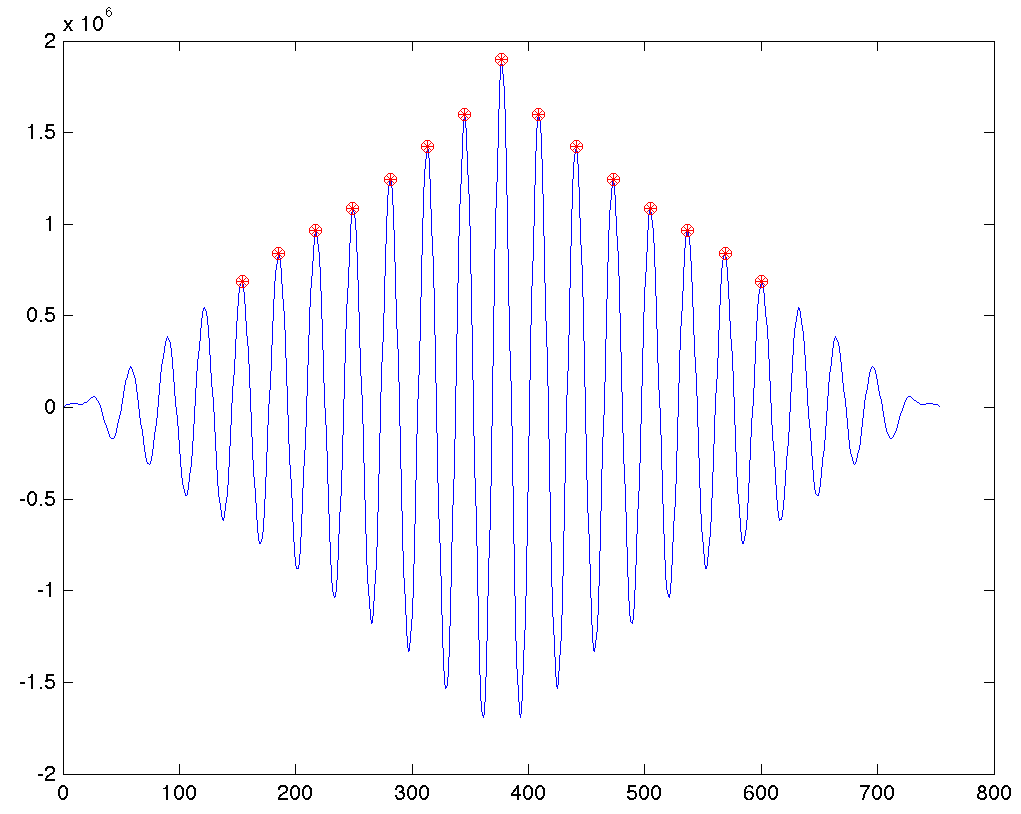
\includegraphics[width=\columnwidth]{textauto.png}%
\subcaption{Text Block: Horizontal Autocorrelation}
\label{textauto}
\end{subfigure}
\caption{Text Block Analysis: a) Text Block b) The horizontal projection with its mean subtracted out of the text block in part a c) the autocorrelation of the horizontal projection with the border effects removed}
\end{figure}

While designing the classification step, it was observed that the horizontal projection near the top and bottom border of a text block negatively effected the classification step; so in each projection, the ends are removed. The edge removed projection is the red plot in Figure \ref{texthist}. The details of this are not crucial so further explanation is not needed.


Instead of analyzing the raw signal to determine it's fundamental frequency, it is easier to analyze the autocorrelation of the signal. This is because the autocorrelation of a periodic signal is again periodic. Another reason the autocorrelation is preferred is because the autocorrelation is essentially a summation of many random variables and this essentially smoothes\footnote{By convolution.} the data. Taking a Fourier Transform is the natural next step, however in this project, the fundamental frequency was calculated in the primal domain by finding the mode distance between a subset of the most significant maxima, which offered a more robust way of rejecting figure blocks. Figure \ref{textauto} shows an example of the autocorrelation of a horizontal projection with marks on the most significant peaks.


If the autocorrelation did not have enough significant maxima to establish a fundamental frequency/period, then the block was classified as a figure. As a comparison, Figure \ref{figfigure} shows the autocorrelation of a figure's horizontal projection with the most significant peaks marked.


\begin{figure}%
\setcounter{subfigure}{0}
\centering
\begin{subfigure}{.33\columnwidth}
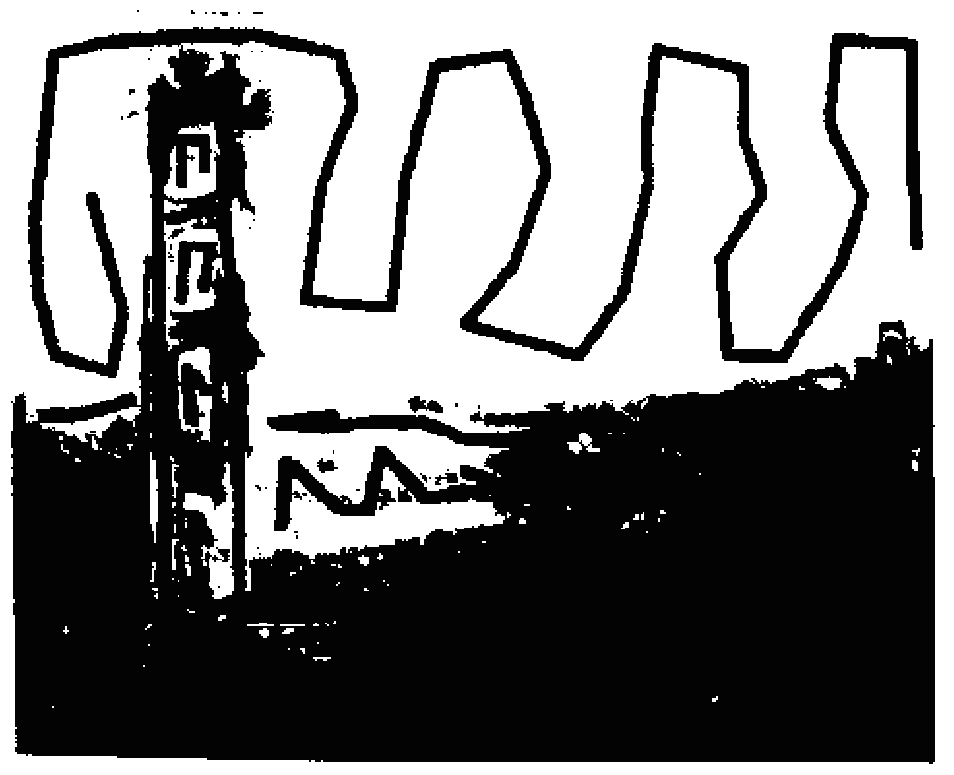
\includegraphics[width=\columnwidth]{figblock.png}%
\subcaption{Figure Block}
\label{figblock}
\end{subfigure}\hfill%
\begin{subfigure}{.33\columnwidth}
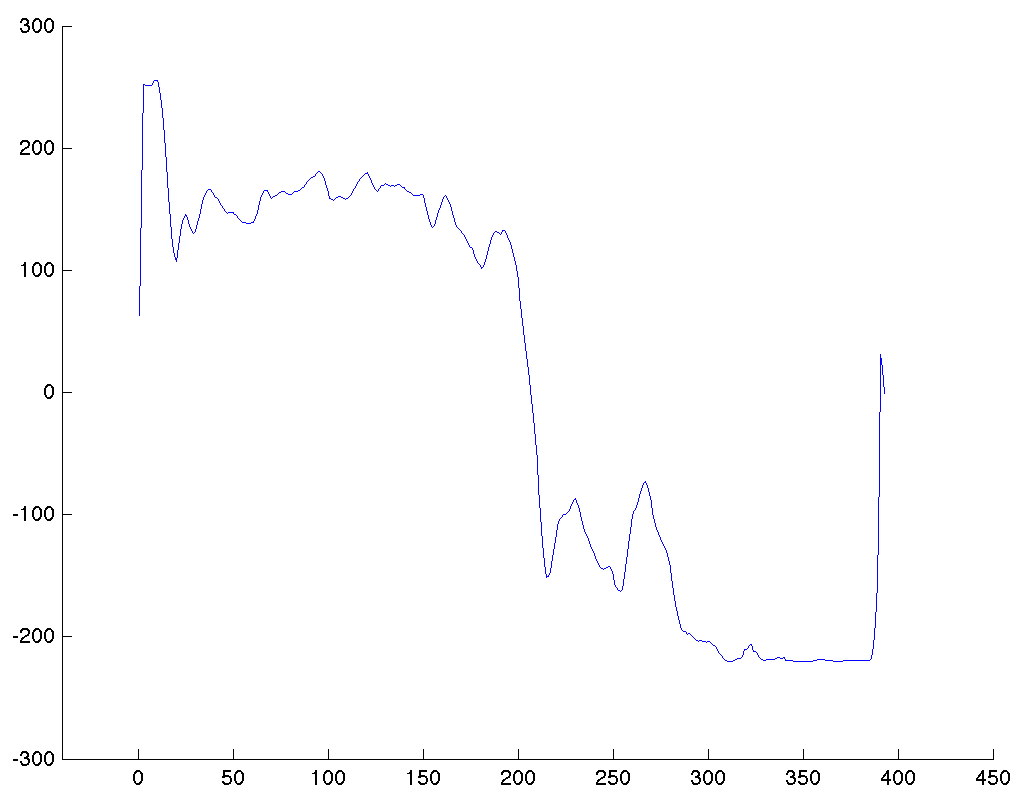
\includegraphics[width=\columnwidth]{fighist.png}%
\subcaption{Figure Block: Horizontal Projection}
\label{fighist}
\end{subfigure}
\begin{subfigure}{.33\columnwidth}
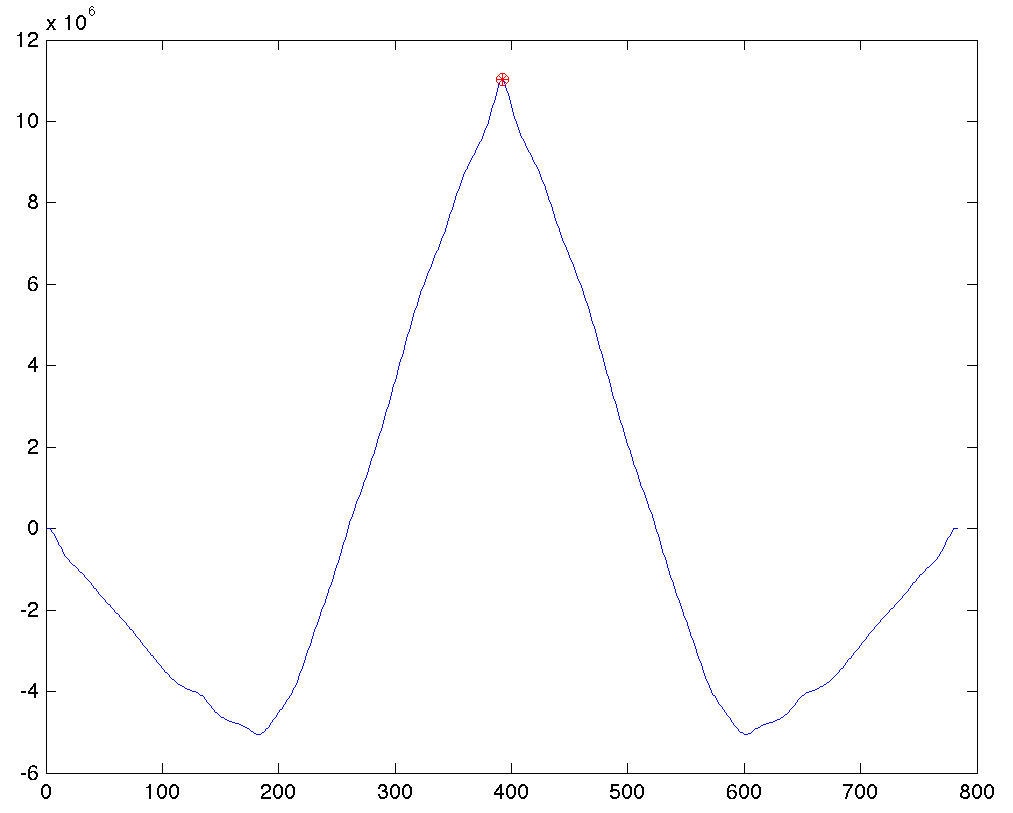
\includegraphics[width=\columnwidth]{figauto.png}%
\subcaption{Figure Block: Horizontal Autocorrelation}
\label{figauto}
\end{subfigure}
\caption{Figure Block Analysis: a) Figure Block b) The horizontal projection with its mean subtracted out of the text block in part a c) the autocorrelation of the horizontal projection with the border effects removed}
\label{figfigure}
\end{figure}


This use of the autocorrelation to classify large text blocks is robust against slight variations in skew angle. This is because the horizontal projection is still quasiperiodic because of the periodicity of the line breaks. This is shown in Figure \ref{textskew}.

\begin{figure}%
\setcounter{subfigure}{0}
\centering
\begin{subfigure}{.33\columnwidth}
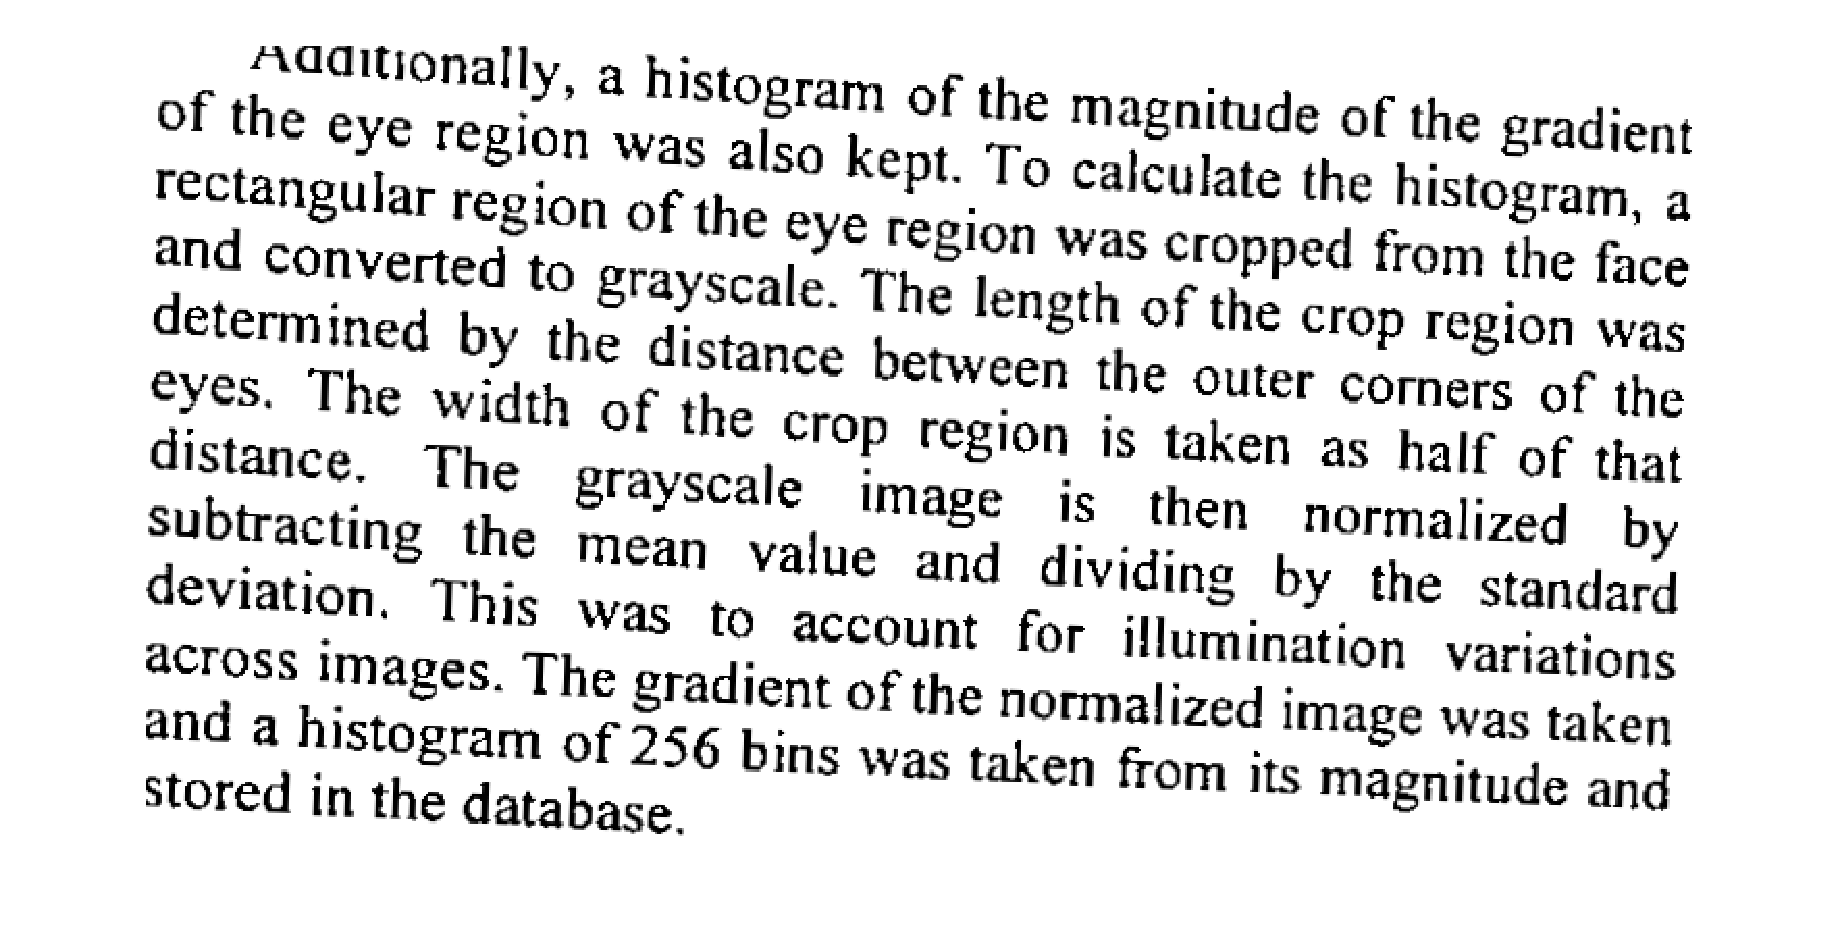
\includegraphics[width=\columnwidth]{textblockskew.png}%
\subcaption{Text Block with Skew}
\label{textblock}
\end{subfigure}\hfill%
\begin{subfigure}{.33\columnwidth}
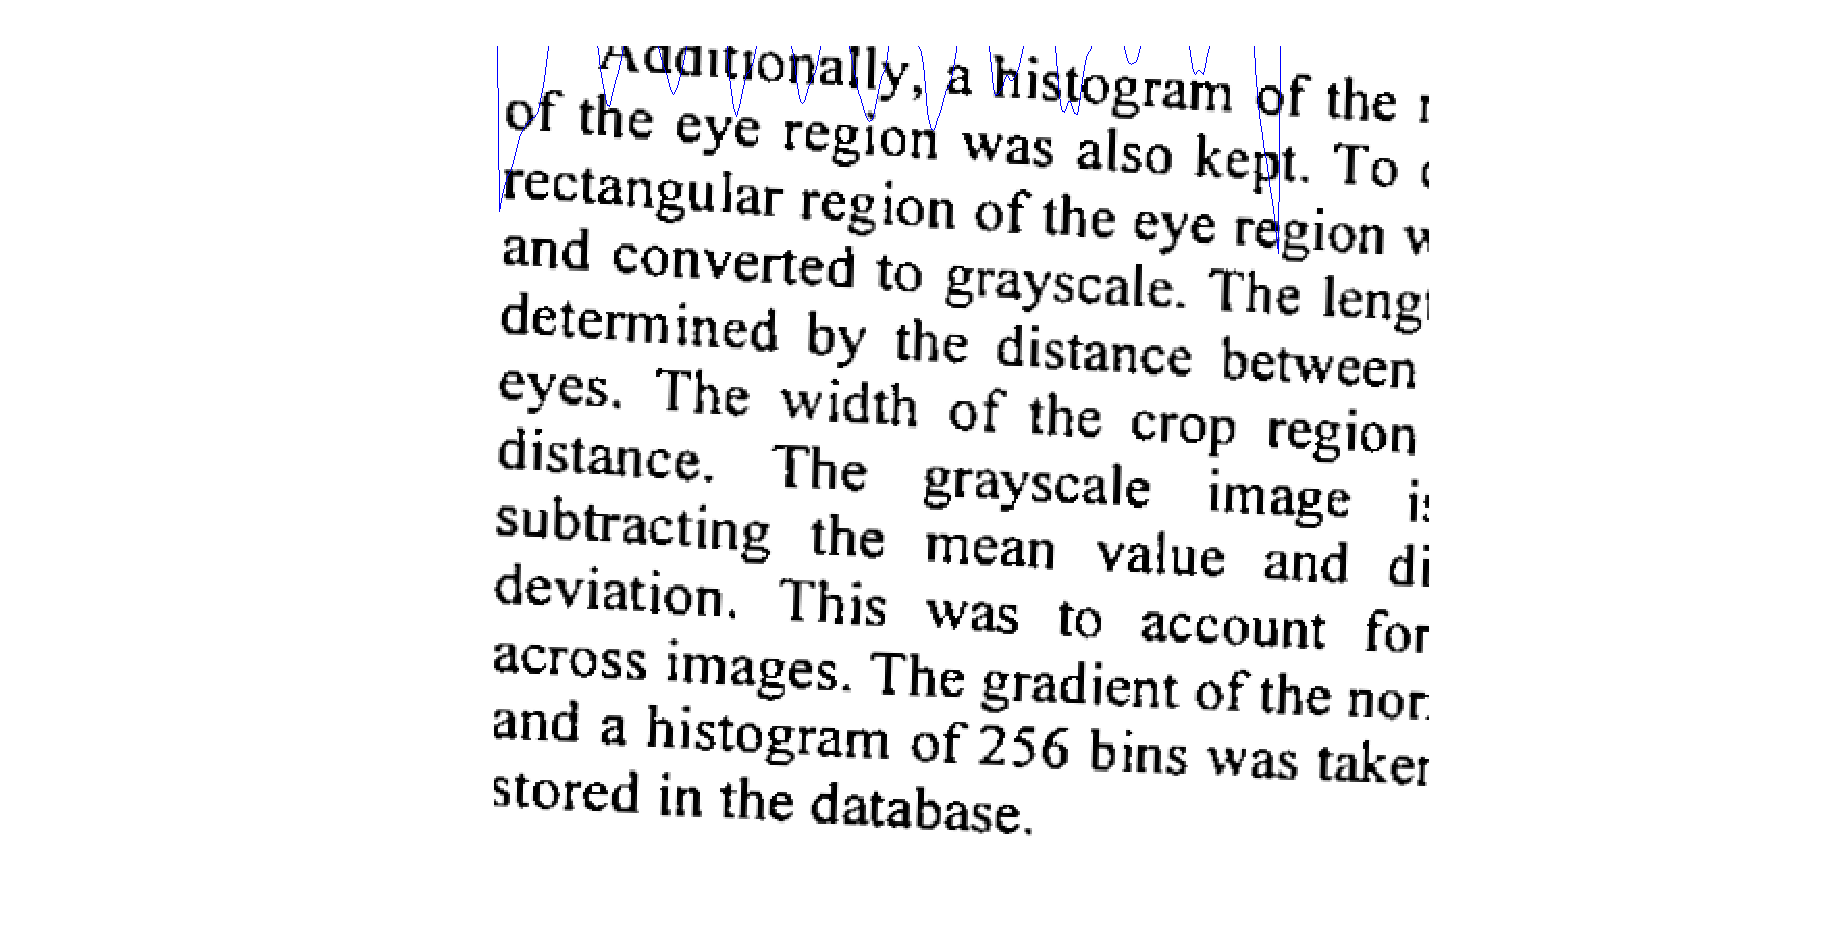
\includegraphics[width=\columnwidth]{texthistskew.png}%
\subcaption{Text Block with Skew: Horizontal Projection}
\label{texthist}
\end{subfigure}
\begin{subfigure}{.33\columnwidth}
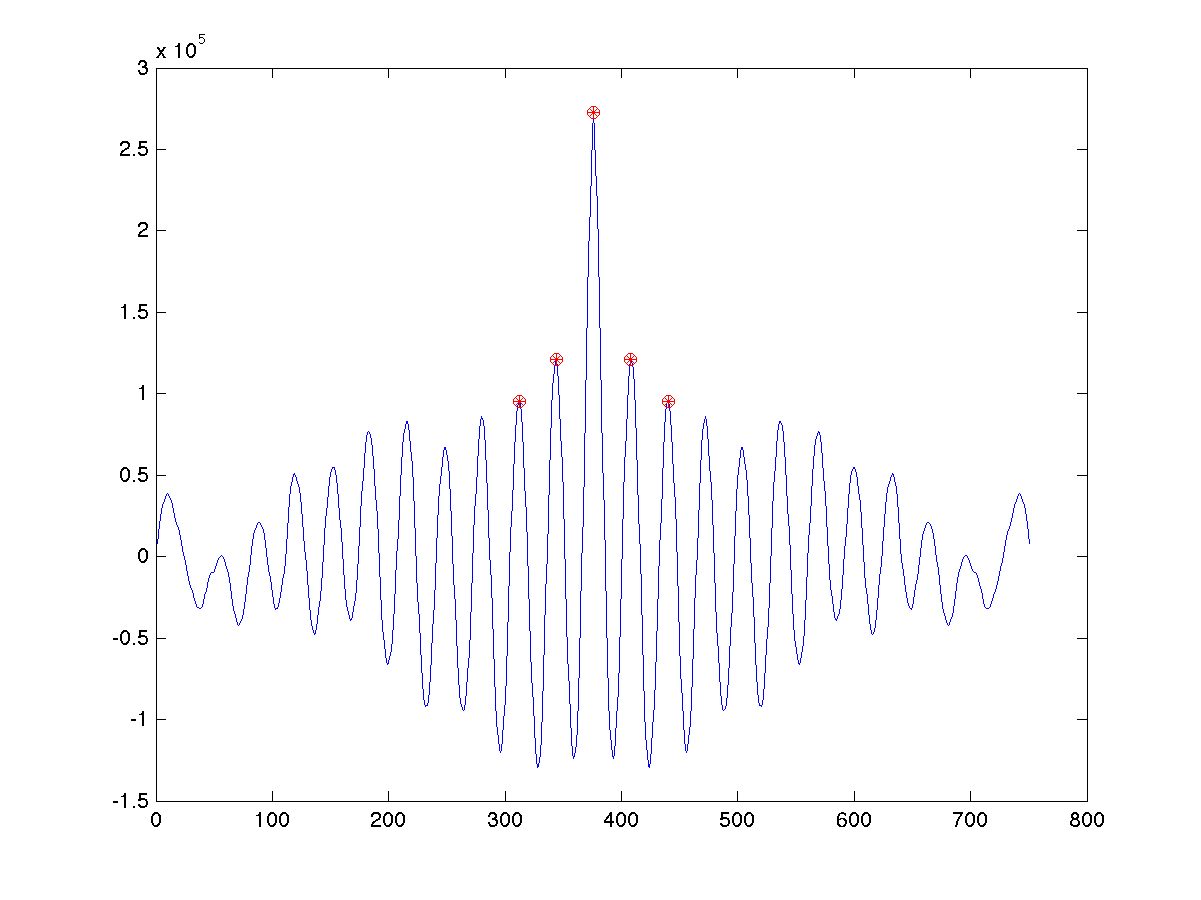
\includegraphics[width=\columnwidth]{textautoskew.png}%
\subcaption{Text Block with Skew: Horizontal Autocorrelation}
\label{textauto}
\end{subfigure}
\caption{Text Block with Skew Analysis: a) Text Block with Skew b) The horizontal projection with its mean subtracted out of the text block in part a c) the autocorrelation of the horizontal projection with the border effects removed}
\label{textskew}
\end{figure}


\subsubsection{"Small" Blocks}
To classify smaller blocks, the approach involved categorizing each block by its area, aspect ratio, and vertical projection to surmise the type. This idea isn't completely new and still appears in the literature \cite{Classification} as a reasonable approach when the classification problem has a narrow scope.

The rules that were implemented in this project were:

\begin{itemize}
\item If the height of the bounding box\footnote{The convex hull of a connected component from the MWR mask} is shorter than some threshold it is not a figure.
\item If a small block in area has a large aspect ratio it is either a line of text or a horizontal divider depending on the variance of its vertical projection.
\item If a block has small area and close to unity aspect ratio, it is either text, like a page number, or part of a figure.
\end{itemize}


These rules are not meant to comply with every document layout; however, for the document layouts of interest, these rules seemed to work well.


\subsection{Local Classification}
Once all of the blocks are classified as text, figure, or neither, we can double back and further determine what kind of text blocks we have. This is important since our goal is to classify document parts with fine granularity to make the layout classification task easier. Another advantage to doubling back is that content such as figures that do not have captions underneath them must have been incorrectly classified in the global-to-local classification step. This improves the accuracy of classification.


The rules that were implemented in this project were:

\begin{itemize}
\item Captions must appear proximal and below a figure. There can only be one caption per figure.
\item Page numbers are "small" blocks of text that are centered with respect to the entire page and must be below a certain point on a page. The fact that they are "small" blocks prevents misclassification of a footer.
\end{itemize}

Footers were not classified since they are usually separated from text by a horizontal line. If the skew of the binary document is incorrect, without OCR, this horizontal line will not be distinguishable from text using only a horizontal or vertical projection.

\chapter{Results}
Since the image pipeline involves executing Matlab code, it was a logical choice to run the image processing off the device. With the current implementation in Java and Matlab running on a 2.3 GHz Intel Code i7, a typical picture of a document taken on an 8MP camera takes approximately 25 seconds to process. The results of 73 pictures of documents conforming to the IEEE conference format are compiled below in Figure \ref{accuracy}. \footnote{Paragraphs were considered as one block and if all lines of text within a paragraph were classified as text, the paragraph was considered correctly classified.} The numbers on top of each bar are the number of document,s out of 73, that contained that content type.
\begin{figure}[h]
\centering
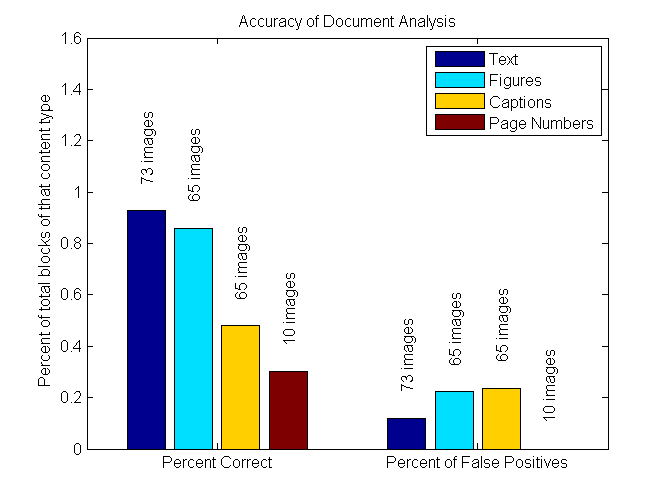
\includegraphics[width = 0.8\columnwidth]{accuracy_report2.png}
\caption{Tested Accuracy}
\label{accuracy}
\end{figure}


\chapter{Conclusions}
As the results suggest, text is the most correctly classified content block owing to the fact that the priority of the classification step is determining whether or not a block is text with the autocorrelation method. The bias in the design of the classification algorithm led to the bias in the results. The classification could be made even more robust if an OCR engine was used to confirm the character components in text blocks, which suggests a route for future work.


Another observation was that the accuracy was heavily dependent on the skew estimation in the preprocessing step. While the classification step may still be correct if a block is slightly skewed, the maximal white rectangle analysis may not return maximal rectangles that segment content properly. This is a huge contributor to the error observed in Figure \ref{accuracy}.


Future work for this project includes developing a bottom up approach incorporating OCR to transcribe the text in each text block as well as produce the \LaTeX code that creates the layout of the document.

\begin{thebibliography}{9}

\bibitem{BairdOrig}
Baird, H.S., "Anatomy of a versatile page reader," \emph{Proceedings of the IEEE}, vol.80, no.7, pp.1059,1065, Jul 1992

\bibitem{Classification}
Gupta, G.; Niranjan, S.; Shrivastava, A.; Sinha, R., "Document Layout Analysis and Classification and Its Application in OCR," \emph{Enterprise Distributed Object Computing Conference Workshops, 2006. EDOCW '06. 10th IEEE International}, vol., no., pp.58,58, 16-20 Oct. 2006

\bibitem{MWRarticle}
H. S. Baird, S. E. Jones, and S. J. Fortune, ?Image segmentation using shape-directed covers,? in \emph{Proc. IAPR IOth Int. Conf: Pattern Recognition}, Atlantic City, NJ, June 17-21, 1990.

\bibitem{art1}
Cattoni, R., Coianiz, T., Messelodi, S., & Modena, C. M. (1998). Geometric layout analysis techniques for document image understanding: a review. \emph{ITC-irst Technical Report}, 9703(09).

\bibitem{art2}
Nazemi, A., Murray, I., & McMeekin, D. A. (2014). Practical segmentation methods for logical and geometric layout analysis to improve scanned PDF accessibility to Vision Impaired. \emph{International Journal of Signal Processing, Image Processing and Pattern Recognition.}

\bibitem{lec1}
B. Girod, "Image Segmentation" [Lecture Notes]. April, 2014.

\bibitem{lec2}
B. Girod, "Edge Detection" [Lecture Notes]. April, 2014.

\bibitem{lec3}
B. Girod, "Morphological Image Processing" [Lecture Notes]. April, 2014.

\end{thebibliography}



\end{document}
